\documentclass[10pt,a4paper]{article}
\usepackage[margin=1.2in]{geometry}
\usepackage{times}
\usepackage{graphics}
\usepackage{graphicx}
\usepackage{natbib}
\usepackage{durhampaper}
\usepackage{subcaption}
\usepackage{caption}
\usepackage{todonotes}
\usepackage{glossaries}
\usepackage{booktabs}
\usepackage[font=small,labelfont=bf, textfont=it]{caption}
% \usepackage{harvard}
\usepackage[moderate]{savetrees}
\usepackage{url}
\usepackage{amsmath}

\makeglossaries
\title{Facial Liveness Testing: an approach for the web}
\author{} % leave; your name goes into \student{}
\student{Ryan Collins}
\supervisor{Prof A. Krokhin}
\degree{MEng Computer Science}

\date{\today}

% Now the main body of the document.
\begin{document}
\maketitle
\begin{abstract}
% These instructions give you guidelines for preparing the final paper.  DO NOT change any settings, such as margins and font sizes.  Just use this as a template and modify the contents into your final paper.  Do not cite references in the abstract.
% However, with facial recognition comes face spoofing: methods to fool the algorithms into thinking one is someone different to who they are.
% The abstract must be a Structured Abstract with the headings {\bf Context/Background}, {\bf Aims}, {\bf Method}, {\bf Results}, and {\bf Conclusions}.  This section should not be longer than half of a page, and having no more than one or two sentences under each heading is advised.
\paragraph{Context}
With password-based authentication methods being subject to many attacks, facial recognition is an alternative, relying on biometrics rather than remembering an easily stolen string of characters.
Existing facial recognition systems remain vulnerable to spoofing attacks, which compromise the security of the system. The solution is to use liveness tests, to determine whether the person behind the camera is real, and not an image or video. The future of face recognition is dependent upon facial liveness tests, to detect impersonation. 

The liveness tests of the future require a standardized input, which can use existing hardware. Furthermore, these liveness tests need to be fast to execute.

In addition, a module is needed to allow multiple liveness tests to work together to yield a single liveness value.

This project developed several new liveness tests to meet these requirements. A module to fuse liveness tests together is also produced, with more testing on more liveness tests required.

\paragraph{Aims}
    % This might belong more in the method.
    \begin{itemize}
        \item To design, implement, train, and test a new quality based facial liveness test for classifying a whole image.
        \item To design, implement, train, and test a new facial feature based liveness test, using Residual Networks.
        \item To design, implement, train and test a new 3D based mask attack detection liveness test using 2D to 3D reconstruction methods.
        \item To design and test a method for combining multiple liveness tests into one single metric to measure liveness, that can be used to include further liveness tests.
        \item To only consider liveness tests that can be used on a mobile device, containing a camera of varying quality, and other IoT devices. No special hardware must be necessary to collect the required data.
        \item To develop liveness tests that can classify liveness for a single image in a maximum of 2 seconds.
    \end{itemize}

\paragraph{Method}
    This project involved the design, training, and testing of three different innovative liveness tests. 
    The NUAA and Replay-Attack devel datasets were used for training, with the Replay-Attack test dataset being used for testing.
    
    The first test developed was the W-IQA liveness test. This analysed image quality across the entire image, using
    a combination of 24 different image quality metrics with a Linear Discriminant Analysis classifier (LDA) to predict liveness.

    The second test developed was the CNN based 2D liveness test. This model used a CNN-based face extraction process to obtain the input face, before feeding this through a ResNet50 based model to classify whether a specific face was real or spoofed.

    The third was a 3D based liveness test to detect mask attacks. This process combined existing techniques for reconstructing a face in 3D from a 2D image, and fed this reconstruction through a VoxNet classifier to detect whether the 3D data contained spoofed input or real input.

    Using the classification probabilities from liveness tests, an LDA based classifier was then trained to fuse the results of the above metrics together, to improve accuracy and allow for future expansion with further liveness tests. this layer also would allow easier access by external systems, dealing with a single definitive liveness metric, rather than many.
  
\paragraph{Results}
2D attacks were tested using the Replay Attack test dataset. Top-1 accuracy was measured to determine overall performance. 

The W-IQA test performed admirably, producing an 87\% accuracy. When this test produced errors, false positives were more common. As a result, spoofed images were classed as real.

The CNN based 2D liveness test performed adequately, yielding a 71\% top-1 accuracy. When this test produced errors, false negatives were far more common. As a result, fewer security concerns were generated by incorrect predictions.

The 3D based liveness test performed poorly. Real-time performance of the model far exceeded the 2-second requirement. The model also required large amounts of memory, leading to training problems. This liveness test is not feasible for use in a real-time liveness system.

A consolidation layer was designed, based on the LDA classifier. Liveness tests yielded linearly separable properties when combined, resulting in improved LDA performance. Future work is needed to test this consolidation layer on more liveness tests, as two metrics isn't enough to justify the benefits of an LDA.

\paragraph{Conclusions}
W-IQA and 2D CNN liveness tests showed promising results for inclusion in a real-time liveness system. Prediction time for both tests was within a 2-second limit. Both tests required no special hardware.

The W-IQA test produced excellent accuracy scores but was let down by false classification of spoofed images as real. Resolution differences also led to performance problems. This model would be improved by utilizing data with different resolutions.

The 2D CNN test produced satisfactory accuracy scores but showed impressive caution at classifying faces correctly. Future work should improve the datasets used, to guarantee each image has a detectable face.

The 3D mask attack detection test performed poorly due to tremendous memory requirements. 2D to 3D reconstruction time also took longer than the required time for a single prediction. This liveness test is not suitable for real-time liveness prediction.
\end{abstract}

\begin{keywords}
Facial liveness, convolutional neural networks, image quality metrics, residual networks, anti-spoofing
\end{keywords}

\section{Introduction}
    Facial recognition is becoming an increasingly popular method for authentication. However, these methods still have opponents. Adam Schwartz, a lawyer with the Electronic Frontier Foundation,  criticized these methods by saying "We can change our bank account numbers, we can even change our names, but we cannot change our faces.
    And once the information is out there, it could be misused". \cite{NPRArticle}

    For facial recognition to become more widespread, methods of detecting spoofing are necessary, to ensure stolen identities can't easily yield security problems. Liveness systems are the answer to this problem. 

    While different methods of detecting liveness are available, these are specialized towards defending against a different type of attack.
    Some existing liveness tests require the use of specialized hardware or sensor configurations that are not available in most smartphones/computers. 
    This work aimed to develop liveness tests requiring a single camera as input. The proposed liveness tests were required to produce predictions in near-real time (2 seconds) with sufficient accuracy.
    This work also proposed a method of fusing liveness test results to produce an absolute liveness value, for use within recognition applications.
    Future extensions could apply the tests proposed here for applications within web-based or internet of things (IoT) applications. 

    In this context, a new 2D CNN based liveness test was proposed, used to analyze 2D facial images for liveness. An existing quality-based test was also modified to provide liveness scoring based on image quality. For 3D based mask attacks, a new liveness test was also developed based on a 2 part approach: (i) VRN based 3D reconstruction (ii) VoxNet based 3D classification.

\section{Related Work}
    As defined in \cite{FaceSpoofingAttacksStudy}, there are three common types of spoofing attack: Photo Attack, Video Attack, and Mask Attack.
    Photo and Video attacks are both classed as 2D spoofing attacks, while mask attacks are 3D attacks.

    \subsection{2D Spoofing Attacks}
        2D based attacks rely on presenting a previously retrieved photo/video, on some medium, to the camera input. Photo attacks rely on a single printed photo being presented. Video attacks consist of a video being played back on a screen. \cite{FaceSpoofingAttacksStudy}
        
        The different methods of liveness tests are shown the the following sections.

        \subsubsection{Video-based tests}
        

        Since video consists of multiple frames, motion can be used to determine liveness. 

        \paragraph{Depth-based liveness}

        The method proposed in \cite{SFMClassifier} uses a structure from motion (SFM) process to reconstruct a person's face in 3D and uses depth information to consider whether the person is real. The process then extended this by fusing depth information with audio verification to improve the prediction results, using a Bayesian network. \cite{SFMClassifier} While this worked with large amounts of motion, running SFM on a video with little motion yields a result with little depth. Another drawback was the requirement for video input since video capture is more time consuming and more challenging.
        
        \paragraph{Blink Detection}
        The blink detection test analyses natural video input to determine whether blinking has occurred. Unlike other video-based methods, this looks for natural behavior rather meaning the user isn't required to carry out any motion. \cite{BlinkDetectionLivenessTest} 
        However, this test can be easily defeated by making eye holes within a printed picture. 
        Furthermore, investigating this liveness method is difficult due to the shortage of video data available.
    
        % Face Flashing
        \paragraph{Face Flashing}
        Possibly the most promising video-based liveness detection test, this method relies on a screen acting as a light source and considering the color and reflective properties of light. Light reflects differently off a face compared to a piece of paper/mask, and therefore the light reflections can give an indication into liveness. Different colors can also be used to add an element of randomness, requiring specific color patterns to be detected. Flashes also occur with different temporal patterns, yielding an additional expected metric.

        While incredibly promising, this method requires the use of a screen. While screens are a common component in smartphones and computers, they are less commonplace in some IoT devices. 

        Furthermore, testing this method would be difficult, as existing datasets don't contain any flashing information required. 

        However, in the future, this method could be implemented to add further security into a facial liveness system on the web, where video input is available.
        
        \subsubsection{Quality-based tests}
        When presenting another medium to a camera, there will be a loss in the resultant image, since printers can't replicate all details, and neither can screens. Therefore, by measuring the image quality of an input image, one could train a classifier to predict liveness.

        One existing method utilized this premise by using the result of 25 different image quality metrics to classify realness using a Linear Discriminant Analysis (LDA) classifier. The results were impressive, 
        yielding very little error (3\% on the iris dataset, no error was given for the facial liveness attempt). The overall method was applied to multiple different types of biometric data, but with facial information the facial data was used, containing very little background information. \cite{ImageQualityAssessmentTest}
        By adding background information, it might be possible to detect further quality differences elsewhere. 
        
        Overall, there is a benefit of fusing results together using a classifier. This same method could be adapted to combine the results of multiple liveness tests together.

        \subsubsection{Deep Learning Liveness Tests}
        \todo{Fill in.}
        % Several different existing networks exist.
        % However, work in this space could be improved, and to do this an understanding of the models is required.

        \subsubsection{Neural Networks, and their structure}
        Developing a custom deep learning model requires an understanding of deep neural networks. These consist of many different layers, each linked by weights. Deeper neural networks have recently allowed for more accurate models. Therefore, an understanding of layers is vital.

        \paragraph{Fully connected layers} Fully connected (or dense) layers consist of neurones. Given two layers $l_1$ and $l_2$, each
        neuron $n_i$ in $l_1$ is linked to each neuron $n_j$ in $l_2$ with a weight $w_{i, j}$. For each neuron in the previous layer, the output of that neuron is multiplied by a weight, the total is summed,
        and the sum is put through a function $t(x)$ which is the activation function. Examples of activation functions include \emph{reLU}, \emph{sigmoid}, and \emph{hyperbolic tangent}.
        $$n_j = t(\sum_{i \in PrevLayer}(n_i * w_{i, j}))$$

        \paragraph{Convolutional layers} Designed primarily for images, these convolve over an image with a kernel. For each location over an image, the weights are multiplied by the image input at that particular location. These are then fed through an activation function.
        The output of a convolutional layer would be a multidimensional tensor. While 2D images are primarily used for input, 3D convolutional layers follow this same process for 3D representations. 
        Convolutional layers are better suited for images compared to fully connected layers, since fewer weights (also known as parameters) are required, thus reducing the required computation and storage. I believe CNNs provide a key approach to facial liveness since they can be used to learn a variety of features including face structure,
        texture, and other potentially suspicious visual glitches which would be obtained with face spoofing.

        \paragraph{A note about parameters}
        Parameters are a measure for how complex a network is, and therefore how difficult training and prediction is. It's an indication of how large the model needs to be. Parameters define how many connections exist within the neural network.

        \paragraph{Cross-Database Approach}
        While using one dataset can be suitable, using multiple datasets can allow a model to be better at predictions on unseen data (better at generalising). This is the method used in \cite{Patel2016CrossDatabaseFA}, which utilises multiple datasets to improve the amount of training data available, and to provide a completely independent test dataset.
        This method also fuses mulitple methods together, to further analyse quality using a CNN, ensuring the features can be
        more easily learned. The drawback with this method however is the large amount of convolutional layers that are required. 
        
        \subsubsection{General 2D image classification models}
        The process of facial liveness can be considered an image classification problem. 
        While previous works have focused on developing new methods to solve the liveness problem, a prudent approach might be to apply an existing image classification model to the problem. 
        Recent research into visual object recognition has led to the development of different neural network architectures, which have gained excellent results in solving this problem.
        Many of these architectures also operate with reasonable computational requirements.
        These models use a dataset called the ImageNet dataset, which contains images separated into 20,000 categories. However, some variations exist with fewer categories.
        These different models include:
            
            \paragraph{AlexNet} 
            This model contains 5 convolutional layers and 2 fully-connected layers, with additional max-pooling layers to reduce dimensionality. 
            This model was used to classify 1.3 million high-resolution images into 1000 classes. \cite{AlexNet} 
            With a low number of parameters, AlexNet is fairly easily deployed (since fewer computation resources are required). Figure \ref{Top1AccuracyOverOperations}
            shows that AlexNet requires very few operations, in the range of $<10$ G-Ops. 
            One drawback to AlexNet is the functionality: top-1 classification accuracy isn't as high as more recent methods. As a result, this isn't the most suitable model to use.
            \cite{DeepNeuralNetworkDeployability}
            
            \paragraph{VGG16 Network}
            VGG consists of blocks containing two convolutional layers with fewer filters, and a max pooling layer.  This yields greater liveness prediction results as opposed to AlexNet but requires far more processing power.
            In total, VGG contains 128 million parameters (weights), therefore requiring a large amount of memory and processing power to train, and make a single prediction. 
            \cite{DeepNeuralNetworkDeployability} 
            
            Due to these high computational requirements, this model isn't the most suitable for a real-time system.

            \paragraph{GoogLeNet Inception}
            
            GoogLeNet is an improved module that approximates a space Convolutional Network with a feed-forward construction. One of the major features of GoogLeNet is the Inception module.
            Naively, this inception module requires input from the previous layer, and calculates a 1x1, 3x3 and 5x5 convolution simultaneously, along with a 3x3 max pooling, before feeding all of these outputs into the filter concatenation step. 
            This naive implementation isn't as efficient. Efficiency can be improved by reducing dimensionality. The solution is to apply a 1x1 convolution before each 3x3 and 5x5 convolution, after the max-pooling output. 
            These inception modules can be used and stacked to improve performance without a huge increase in computation. \cite{GoogLeNet} 
            
            Comparatively, GoogLeNet produces improved top-1 accuracy scores compared to AlexNet, as shown in Figure \ref{Top1AccuracyOverNetwork}. 
            GoogLeNet also produces similar results to the VGG model.

            There have been several different version of GoogLeNet. Analyzing the data shown in Figure \ref{Top1AccuracyOverOperations}, more recent versions 
            have yielded improved accuracy characteristics; the Inception-4 model produced the best accuracy scores out of all the ImageNet classifiers. However, 
            this improved accuracy increases the number of operations required. Older versions of GoogLeNet required $<10$ G-Ops, while Inception v-4 required $~18$ G-Ops.
            Compared to VGG, this model performs well, but Residual Network models arguably provide a better balance between accuracy and computational requirements.
            
            \paragraph{Residual Networks}
            Residual Networks (ResNets) aim to improve traditional convolutional networks by reducing the vanishing gradient problem, therefore decreasing training time.
            This problem occurs when early layers have a small gradient, which yields even smaller gradients during later layers. 

            Residual blocks, shown in Figure \ref{ResidualBlock}, solve this problem by utilizing shortcut connections during training, allowing gradients to skip layers if necessary. 
            These connectors work by adding their outputs to the stacked layers.

            Figure \ref{Top1AccuracyOverNetwork} shows that this method yields better accuracy than both VGG and GoogLeNet. In terms of computational performance, 
            Figure \ref{Top1AccuracyOverOperations} shows that ResNet50 requires fewer than 10 G-Ops, whilst yielding 76\% accuracy.

            \begin{figure}
                \centering
                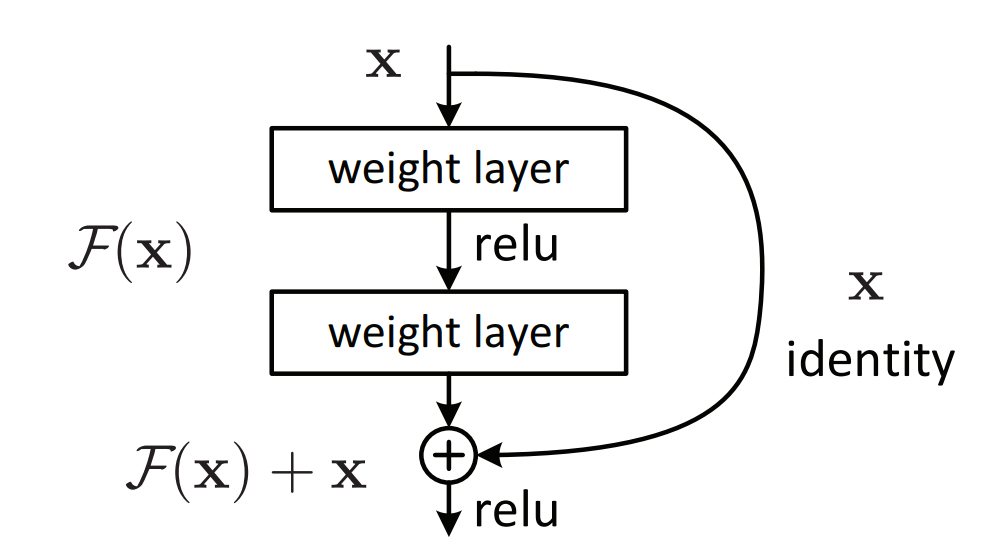
\includegraphics[width=.7\linewidth]{ResidualBlock.png}
                \caption{A Residual Block: this is the building block of the ResNet architecture. Source: \cite{DeepResidualNetworks}}
                \label{ResidualBlock}
            \end{figure}

            \begin{figure}
                \centering
                \begin{subfigure}[t]{.4\textwidth}
                    \centering
                    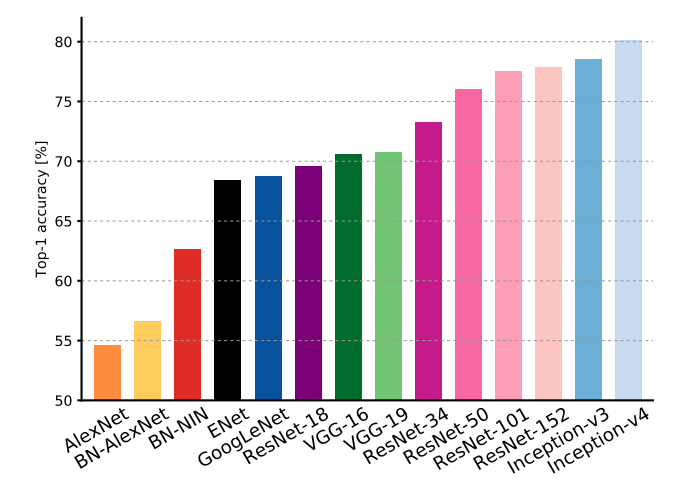
\includegraphics[width=.7\linewidth]{Top1AccuracyOverNetwork.png}
                    \caption{Top 1 accuracy vs network. Chart and results from \cite{DeepNeuralNetworkDeployability}}
                    \label{Top1AccuracyOverNetwork}
                \end{subfigure}
                \hfill
                \begin{subfigure}[t]{.4\textwidth}
                    \centering
                    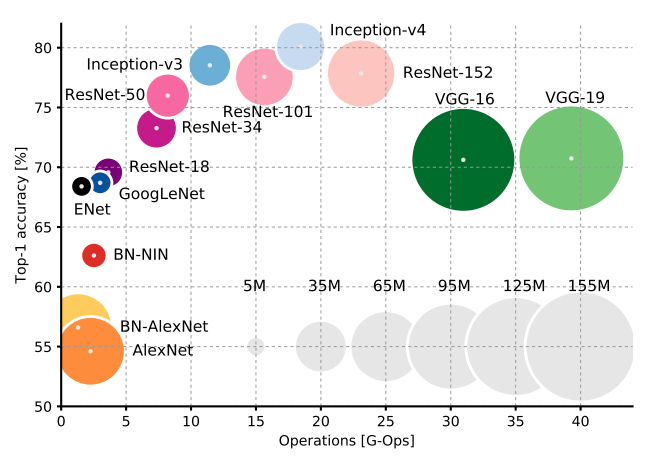
\includegraphics[width=.7\linewidth]{Top1AccuracyOverOperations.png}
                    \caption{Top 1 accuracy vs operations, where network size is proportional to number of parameters. Operations figures are for a single pass (e.g. predicting given a specific input). Chart and results from \cite{DeepNeuralNetworkDeployability}}
                    \label{Top1AccuracyOverOperations}
                \end{subfigure}
                \label{ComparisonsOfDifferentModels}
                \caption{These two charts, from \cite{DeepNeuralNetworkDeployability}, show the accuracy and computational requirements of each type of classifier.}
        \end{figure}

        \subsubsection{Datasets}
        %Datasets
        One of the earliest datasets available for facial liveness was the NUAA dataset. This contained photographs of 15 different subjects, both real and fake images.
         Spoofed images were of paper replay attacks, with the displayed images being both warped and flat. 
         The dataset contained JPEG images with a hierarchical structure. One drawback with this dataset is licensing: the dataset is only available for non-commercial use, 
         such as research purposes. Future, more commercial works, would, therefore, require a different dataset be used in order to meet the licensing objectives. \cite{NUAADataset}

        In 2012, the Replay-Attack dataset was first released, consisting of 1,300 video clips. These video clips contain both real and spoofed data. Spoofed data contains a mixture of different attack methods,
        including printed photograph, video, with both high and low-resolution media. To facilitate training, testing, and validation, the dataset also contains sub-datasets.
        The 'devel' dataset was designed for training and validation purposes, while the 'test' dataset was designed for testing the trained model.  \cite{ReplayAttackDataset}

        While individually, these datasets might not contain enough data, together they provide enough samples to reasonably train and test our models.
        They shall be used throughout this project for both training and testing the 2D based liveness models.

            
    \subsection{3D Spoofing Attacks}
        Mask Attacks are a 3D spoofing attack, which involve creating a 3D mask of someone and wearing it. \cite{FaceSpoofingAttacksStudy} These are much less prevalent, but with 3D printing becoming more mainstream, this
        could potentially get more prevalent in the future.

        % Explain the method shown in Choudhary et al., 1999 - SFM. Problem: depth information ahrd to obtain when still with SFM. Noise also problematic.
        % Which uses Structure From Motion.
        In 2013, the 3D Mask Attack Dataset (MAD dataset) was released. This dataset contains 76500 frames of 17 people, recorded using a Kinect camera.
        Each frame contains a depth image, an 2D RGB image with 8 bit color and a size of 640x480 pixels. Each frame also contains eye positions.
        Real Access samples are contained within the first and second session folders, while the third session contains the frames of mask attacks. The subjects contained
        within each frame are denoted within the filename.
        
        \cite{3DMadDataset}

        \subsubsection{Obtaining 3D data from 2D images/video}
            One method of obtaining 3D data from a video is to use Structure From Motion (SFM). This method was previously utilized in \cite{SFMClassifier} to consider the depth data as a 2D liveness test,
            but this method could potentially work as a solution for obtaining 3D data. However, SFM performs poorly when given a video with a small amount of motion. Furthermore, the 3D mask attack datasets
            available for this project do not contain video but single images, which means such a method would be more difficult to test.

            However, with improved machine learning models, there exist models that can reconstruct facial structure based on a single 2D image. One such model is the VRN model, proposed in \cite{3DReconstructionMethod}.
            The paper, and the associated source code, contains a model that takes a 2D image as input (of size 192x192), and produces a voxel representation of the 3D face structure. This model is more suitable for our
            application, since the use of a 2D image rather than a video works well with the datasets available. Furthermore, use of a single 2D image would require less user input as a SFM based method, since the user isn't required
            to move in order to produce an adequate 3D reconstruction. An example of the 3D reconstruction obtained from this model can be seen in Figure \ref{3DReconstructionScreenshot}. The screenshot is obtained from the GitHub repository
            of a Keras-based implementation of this method (since the initial implementation of the paper used the Torch library).

            \begin{figure}
                \centering
                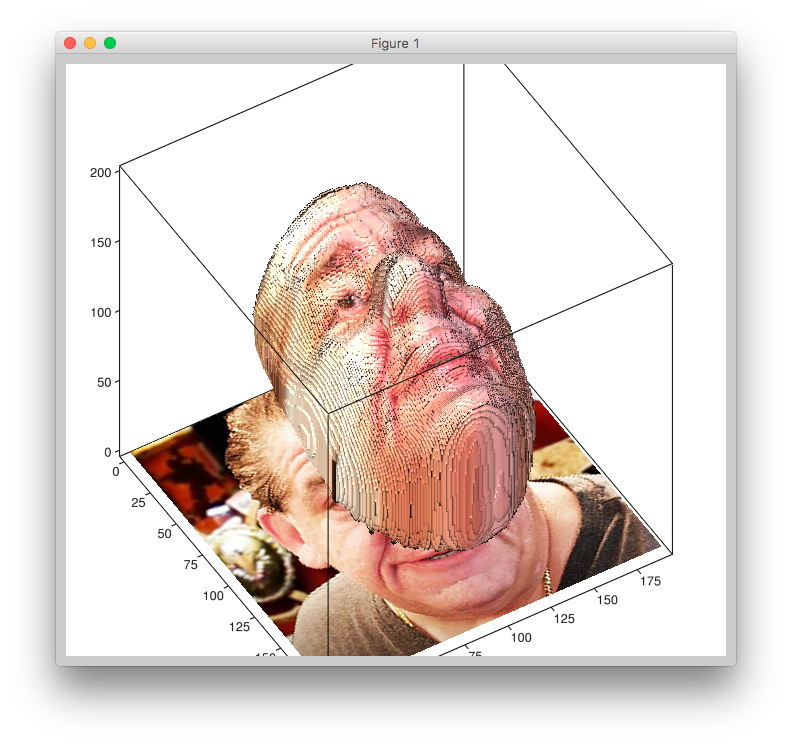
\includegraphics[width=.5\linewidth]{3DReconstructionFromSource}
                \caption{A screenshot from the VRN Torch to Keras version (a conversion of the VRN model to Keras). This screenshot is from \cite{VRNTorchToKeras}}
                \label{3DReconstructionScreenshot}
            \end{figure}

            % \todo{VRN 3D reconstruction on MaskAttackDataset image}

        \subsubsection{3D Classifiers}
            In a similar approach to the 2D methods researched above, there are a variety of existing 3D classifiers that could be re-purposed for the liveness classification approach.
            While these methods don't yield the same accuracy figures as with ImageNet, further improvements in the field of 3D classification could lead to better liveness methods in the future.

            \paragraph{PointNet}
                PointNet is a model for classifying point clouds, represented as an unordered set of points. PointNet in total has 3.5 million parameters, with 440 million FLOPs per sample, which 
                is a reasonable number considering other classifiers, but is on the upper end of what would be expected for a web based system. The classifier used within PointNet is a simple feed forward network.
                \cite{PointNet}
                While this model has performance benefits over CNN based models (since 3D convolution is computationally expensive),
                the input is a point cloud structure which might not be the most ideal solution (since sparse data might not be captured, dependent on which reconstruction model is used).
                
            \paragraph{VoxNet}
                Unlike PointNet, this model uses a voxel representation. This is ideal due to the nature of existing 3D reconstruction models from a 2D image. The accuracy of this classifier isn't the most ideal,
                but improvements could be made such as implementing a Residual network approach (something that worked well for 2D classifiers). As a proof of concept, this model would be ideal to test whether this model would work
                in the real world. This model was developed to identify objects based on their 3D representation.\cite{VoxNetModel} This is very similar to the process of identifying liveness based on the 3D face structure input.
                The overall architecture of the classifier can be seen in Figure \ref{OriginalVoxNetArchitecture}. Convolutional layers are used to learn the 3D feature space, while a dense layer is used to produce the output. 
                \begin{figure}[]
                    \centering
                    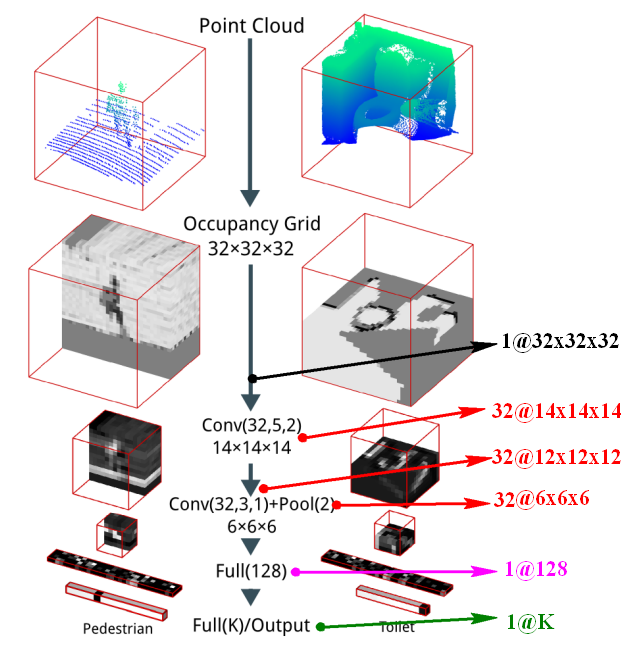
\includegraphics[width=0.5\linewidth]{VoxNetArchitecture.png}
                    \caption{The original VoxNet architecture. While point cloud input is available, voxel based representation can also be used. Diagram obtained from \cite{VoxNetModel}}
                    \label{OriginalVoxNetArchitecture}
                \end{figure}
\section{Solution}
    % Solution to the problem
    \subsection{Specification, and design requirements}
        \begin{enumerate}
            \item \label{SpecPoint1} Any liveness test produced must be able to predict a single image in under 2 seconds on a standard i7-7700k powered machine
            \item \label{SpecPoint2} Any liveness test must only require the use of a 2D image input from a standard built in camera. No other external hardware is allowed.
            \item \label{SpecPoint3} The Top-1 accuracy figure of each liveness test should be greater than 70\%.
            \item \label{SpecPoint4} The liveness test consolidation layer must allow for future inclusion of further liveness tests,.
            \item \label{SpecPoint5} A liveness test should be developed to classify the entire image, to detect spoofing given a specific input.
            \item \label{SpecPoint6} A liveness test should be developed to detect liveness based on the 2D input of a facial area from a camera.
            \item \label{SpecPoint7} A liveness test should be developed to specifically detect 3D based attacks (mask attacks).
        \end{enumerate}

        \ref{SpecPoint1} is important to ensure that the liveness tests that are built don't take too long to execute and yield a result. While in practice an Intel i7-7700k machine might have a
        slightly higher clock speed than a standard cloud-based processor, the results would still be reasonable in practice.

        Some of the liveness tests proposed in previous works require the use of specialised hardware which won't be available on many devices. The most common device capable of taking in facial input is a
        webcam, and since these are found in many laptops, IoT devices, and smartphones, this is an ideal limiting factor. While screens could also be considered useful, certain IoT devices might not necessarily have them either.
        This is what \ref{SpecPoint2} aims to address.

        The results of the liveness tests produced are also important, since a random prediction of liveness yields a 50\% accuracy, so therefore a 70\% accuracy yields a reasonable performance over this, and might require extension to improve it further,
        while a higher accuracy indicates that the liveness test performs better and might have been refined more. This is what \ref{SpecPoint4} addresses.

        \ref{SpecPoint5}, \ref{SpecPoint6} and \ref{SpecPoint7} propose the method which each liveness test uses and how they work functionally. Whole image detection is necessary due to the potentially poor performance of a model to extract a face,
        since it might be ideal to still be able to obtain a liveness value based on the estimate of the image quality itself. Furthermore, while quality is one factor, analysing the facial structure and texture to determine whether spoofing has occured
        is also an important factor. Finally, mask attacks are still not that common, but with the rise in 3D printing technology we could see an increase in them in the future. As such, a method of preventing 3D based mask attacks is necessary.


        With these specifications in mind, the design focused on three different liveness tests: an Image Quality assessment based liveness test, a ResNet 50 based classifier (based on a pretrained ImageNet model),
        and a novel 3D based classifier using 3D facial reconstruction models interlinked with the VoxNet 3D classification model. Each of these liveness tests have some common services that are needed; these include
        reading large datasets without causing resource availability problems.


    \subsection{Shared Services}
        \subsubsection{Dataset Managers}
        In order to assess our liveness tests and train them, dataset managers are needed.

        A generic implementation of a dataset was created as an Abstract Class, which was then extended by the NUAA, Replay-Attack and Mask-Attack dataset managers.
        This generic implementation allows for future datasets to be easily added, and also provides the class definition of what's needed, to help improve the software engineering process.

        The role of a dataset manager is to load in a dataset from a folder structure (which varies between dataset), conduct any basic preprocessing to convert the files into OpenCV images,
        and produce two H5Py Datasets, one for real images, and one for fake images. The dataset manager also allows further customization, to load specific sub-datasets (such as 'devel' or 'test' in the case
        of the Replay-Attack dataset), or load data regarding specific subjects (in the case of the Mask Attack Dataset). The role of the H5Py dataset is to normalize the datasets into a specific format,
        to allow for easier dataset processing.

        In addition to data normalization, it also provided a method of reducing RAM usage, therefore allowing larger liveness test models to be created. This is because data is only fetched when needed
        from the hard drive, rather than loading the entire dataset into RAM at once.

        \subsubsection{Neural Network Infrastructure}
            % Keras to simplify models, tensorflow as the underlying backend.
            % Training machine on Google Cloud, using 64GB RAM, 8 x vCPUs, and an NVIDIA Tesla P100 GPU to improve performance of the training process through parallelism. 
            
            \paragraph{Neural Network Framework} 
            For the 2D and 3D based classifiers, neural networks were to be used. It was decided to use Keras, with the Tensorflow backend, as Keras provides a high level interface to Tensorflow
            and also allows for other backends to be used in the future (which could potentially perform better in different scenarios). The Tensorflow backend was used because of the easy configuration
            with both GPUs and without (simply install tensorflow-gpu for GPU processing, and tensorflow for CPU only processing), depending on the machine being used. A high level interface was necessary
            to avoid boilerplate too, since models would be regularly changed to find the best outcome for each classifier.

            \paragraph{Hardware for training}
            Training the neural network required more processing power than was directly available. Google Cloud Compute Engine was used to provide this processing power, since it's easily accessible and has existing
            deep learning environments with Intel-accelerated mathematics libraries. The Google Cloud instance also provided easy extensibility, since some of the liveness tests required additional tools that could not be easily installed
            on NCC/Hamilton clusters at Durham University. Training was conducted on a VM with 64GB RAM, 8 virtual CPUs with an NVIDIA Tesla P100 GPU being used to accelerate the training process (through parallelism).

            \paragraph{Hardware for testing}
            GPUs are expensive, and therefore if such a system were deployed the cost of GPUs would provide expensive to run. Therefore, a CPU only implementation for the testing was followed, using an Intel i7-7700K (at 4.2 GHz), with
            16GB RAM. Performance metrics were yielded using this hardware to emulate the expected performance and understand which metrics performed best and whether they performed adequately.

        \subsubsection{Image Processing and Computation Management}
            OpenCV was used to manage the processing of images, including the image loading components. This library was chosen for the wide support available, and for the large feature set that it provides (including Gaussian Blurring, some image metrics, and some fourier analysis).
            For the rare occasions where OpenCV didn't have the required functionality, scikit-image provided some operations that were necessary.
            
            Numpy was instrumental in most other computation operations (including image preprocessing, mathematical calculations), due to the large speed improvements provided by the C implementation (compared to Python's slower math libraries).
            Since OpenCV interfaces well with Numpy, no conversion was needed which improved the ease of implementation.


        \subsection{Image Quality Assessment Liveness Test}
            \subsubsection{Overview}
            One common way of detecting liveness is to consider the image quality of the camera input. When a printout/screen is held up to the camera, the facial image
            will have some noticeable differences, specifically in the high frequencies. There might also be some image compression visible in fake images, compared to real ones.
            This is the basis for this method.

            More specifically, the implementation was based on the work contained in \cite{ImageQualityAssessmentTest}. 24 different image quality metrics were implemented,
            with metric values being used as an input to a classifier. From previous work, it has been shown that this metric is accurate (therefore detecting spoofing well), while
            also being fairly fast to compute in terms of time, meeting \ref{SpecPoint3} and \ref{SpecPoint1}.

            The classifier being used for our implementation is Linear Discriminant Analysis (LDA).

            A visual explanation of the method can be seen in Figure \ref{ImageQualityLivenessTestDiagram}. 

            \begin{figure}
                \centering
                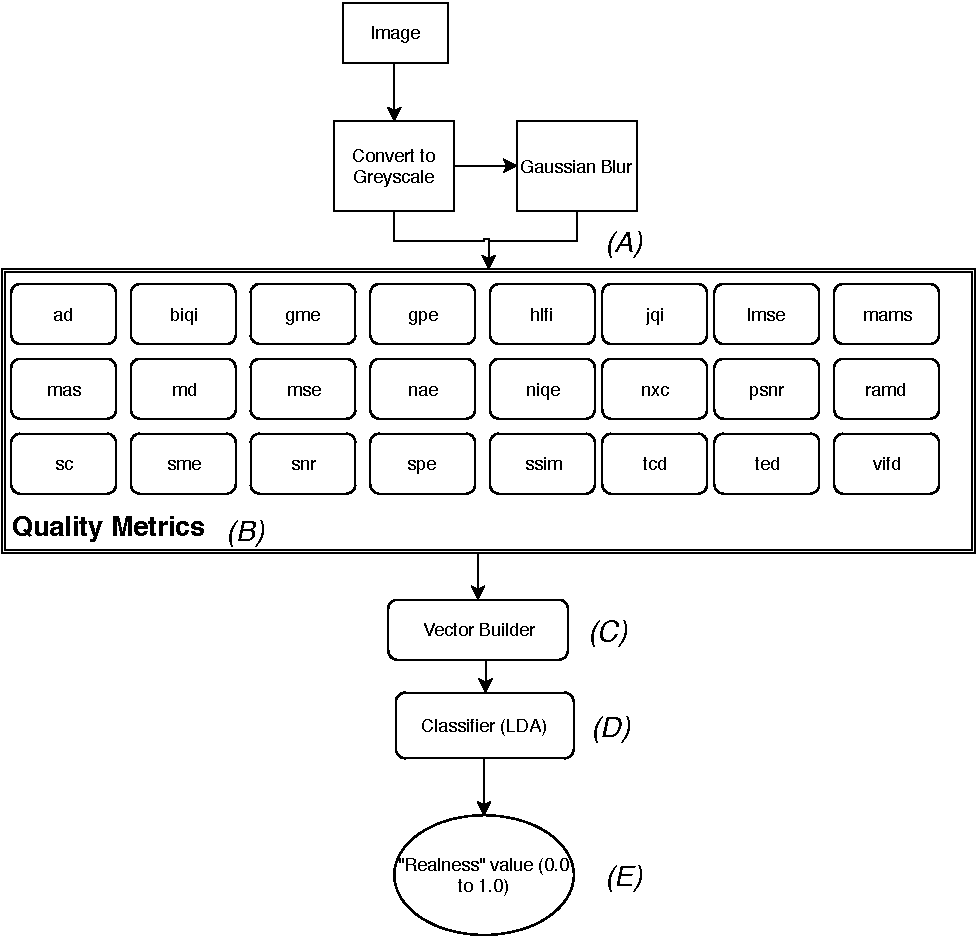
\includegraphics[width=\linewidth]{ImageQualityLivenessTest.pdf}
                \caption{The architecture of the image quality liveness test. (A) The greyscale copy of the image, and a blurred copy of the image are input into each of the metrics.
                (B) The metrics are individually calculated, and a single value output from them. (C) These values build a 1D vector. (D) They are classified using an LDA classifier. (E) The realness value
                is 1.0 for real, and 0.0 for fake, or in between.}
                \label{ImageQualityLivenessTestDiagram}
            \end{figure}
    
            \subsubsection{The Metrics}
            The original paper proposed that 25 metrics were used. However, our implementation used only 24, due to some implementation problems. Most of the metrics were implemented manually as defined
            either in \cite{ImageQualityAssessmentTest}, or utilizing further sources to understand how they worked. In addition, the Matlab source code that was released with \cite{ImageQualityAssessmentTest}
            was referred to, but written manually in Python using Numpy/OpenCV or in some cases other libraries.

            Each of these metrics requires an input image $I$. Non-Reference metrics only require $I$, while Full-Reference metrics require an additional image $I'$. $I' = Gaussian(I)$ in our implementation.
            
            \paragraph{PyVideoQuality Library}
            As part of the implementation process, the NIQE metric required the use of a pretrained classifier which didn't exist for Python. As such, it was necessary to modify existing code.
            The only Python source code available was \cite{VideoQualityOriginal}, which was written for Python 2 and consisted of single Python files that would be difficult to implement into the system.
            As such, the Python 2 code was converted to Python 3 manually, and refactored to follow a python package by myself. This new library was shared-alike, and is now available on GitHub. \cite{VideoQualityUpdated}
            

            \paragraph{Absolute Difference (AD)}
                This is a full reference metric, defined as $AD(I, I') = Mean(I - I')$. This calculation was implemented using Numpy manually.

            \paragraph{Blind Image Quality Index (BIQI)}
                BIQI is a no-reference metric. Rather like NIQE, there was no existing BIQI library implementation. It also consists of a pretrained classifier element, which
                would be hard to replicate without the correct processing or training data. The training set used is the LIVE IQA dataset, which is public domain but requires 
                permission to access which would take quite a bit of time for a small component of the project.

                BIQI consists of two steps: the first is to assess image distortion, and the second is to analyze the quality. 

                As such, an existing implementation was found on GitHub but for Python 2. \cite{BIQIImplementation} This was refactored to work with Python 3, and the code included as part
                of the existing GitHub repository. 

                
            \paragraph{Gradient Magnitude Error (GME)}
                GME is a full reference metric, and it calculates the error corresponding to the gradient magnitude between the two images. The gradients $\Delta I$ and $\Delta I'$
                are calculated using a Sobel filter, kernel size 5 in both X and Y directions. The Sobel filter is calculated using OpenCV within our implementation.

                Using these gradients, the metric is calculated as $GME(I, I') = Mean((\Delta I - \Delta I')^2)$. In our implementation, Numpy is again used to calculate both the mean and
                also the squared difference.

            \paragraph{Gradient Phase Error (GPE)}
                \todo{look into this, because I think GME and GPE might have been switched during implementation for some reason.}
                GPE is a full reference metric, which like GME uses the Sobel filter as a basis. Using four different Sobel filters, gradients in the x and y direction for both
                $I$ and $I'$ are calculated. These are $\Delta I_x$, $\Delta I_y$, and $\Delta I'_x$, $\Delta I'_y$.

                Using these direction gradients, $Mag_{I} = Magnitude(\Delta I_x, \Delta I_y)$ and $Mag_{I'} = Magnitude(\Delta I'_x, \Delta I'_y)$ is then calculated using the gradients shown above.

                Using this, the metric is defined as: $GPE(I, I') = Mean((Mag_{I} - Mag_{I'})^2)$.

            \paragraph{High Low Frequency Index (HLFI)}
                This considers the frequency of specific low and high frequencies within a single image. It is therefore classed as a no-reference metric.
                First, the image is put through a discrete fourier transform process using OpenCV. The frequency spectrum is then shifted and a final magnitude spectrum
                is calculated using Numpy. This magnitude spectrum is defined as $M(i, j)$, where the shape of M corresponds to the image I.

                Using this spectrum, a sum of the low frequencies, from $(1,1)$ up to $(i_l, j_l)$ is calculated by cycling through each pixel in the spectrum. These two upper constants for
                the low frequency band are defined with respect to the shape of M. Given the shape of M is $(X, Y)$, $i_l = 0.15 \cdot X$ and $j_l = 0.15 \cdot Y$.
                For each location (i, j) within the limits, the magnitude spectrum is summed to produce a final value called $lfs$ which is the low frequency sum.

                A similar process is followed for the high frequencies. However, instead of starting at 1, we start from $i_h, j_h$ and finish at $(X, Y)$. The constants $i_h$ and $i_l$ are
                calculated in a similar manner to before, only adding one to the result. Therefore $i_h = Ceiling(0.15 \cdot X + 1)$ and $j_h = Ceiling(0.15 \cdot Y + 1)$, where $Ceiling(x)$ rounds
                a value $x$ up to an integer. The high frequency sum $hfs$ is calculated through this process.

                Based on this, the metric can be defined as $HLFI(I, I') = \frac{lfs - hfs}{\sum_{i,j = 1}^{i,j = (X, Y)} |M|}$.
                
            \paragraph{JPEG Quality Index (JQI)}
                The JQI quality index is used to understand the nature of JPEG compression in an image, specifically with regards to JPEG images being blocky (a nature of the DCT based compression),
                and blurring components (due to high frequency DCT coefficients being lost).

                First the blockiness feature $B$ is calculated as average differences across block boundaries. \todo{EXPLAIN MORE}
                
                Two metrics are then used to define the activity of the image signal. The first is $A$, which calculates the average absolute difference between in block image samples.
                Then, $Z$ is the zero crossing rate. \todo{EXPLAIN MORE WHAT THESE DO}.

                As these above features were calculated individually for horizontal and vertical features, they can now be fused together. This is done simply by averaging them.

                $$B = \frac{B_h + B_v}{2}$$
                $$A = \frac{A_h + A_v}{2}$$
                $$Z = \frac{Z_h + Z_v}{2}$$

                The final calculation uses a number of constants which are defined as:
                $\alpha = -245.8909$, $\beta = 261.9373$, $\gamma_1 = -239.8886$, $\gamma_2 = 160.1664$, $\gamma_3 = 64.2859$.

                Bringing the constants, and the above calculations together, this yields the overall definition of the metric:

                $$JQI(I, I') = \alpha + \beta \cdot B ^{\frac{\gamma_1}{10000}} \cdot A^{\frac{\gamma_2}{10000}} \cdot Z^{\frac{\gamma_3}{10000}}$$

                While other definitions of this can be utilized, this yielded good prediction performance in the paper \cite{JQIPaper}. In our implementation, this was implemented using 
                Numpy.
            \paragraph{Laplacian Mean Squared Metric (LMSE)}
                LMSE is a full reference metric that considers the edge differences to measure quality. A high LMSE value implies that the input image is of poor quality. 
                
                This requires a Laplacian function, which is defined in \cite{LMSEPaper} as:

                $$Laplacian(I(m, n)) = I(m+1, n) + I(m-1, n) + I(m, n+1) + I(m, n-1) - 4\cdot I(m, n)$$

                This function is calculated for each $(m, n)$ in an image. The current implementation uses the above function written in Numpy to produce the Laplacian output. 
                \cite{LMSEPaper}

                Once this operator has been defined, it can then be used to calculate the overall metric: 

                $$LMSE(I, I') = \frac{\sum (Laplacian(I) - Laplacian(I'))^2}{\sum Laplacian(I)^2}$$
                
            \paragraph{Mean Angle Magnitude Similarity (MAMS)}
                MAMS is a full reference metric that considers the similarity between magnitudes of the angles within the image. First, a matrix of scalar products are calculated, such that $S=I \cdot I'$.
                
                Then, a matrix of magnitude products are calculated $M = |I| \cdot |I'|$. All zero values within $M$ are then set to 1, in order to avoid divide by zero errors in a later step.

                Using both $S$ and $M$, the angles at each position on the image were calculated. Each angle produced from the arccos operation is then subtracted from 1. The operation yields a matrix $\alpha$ of angles in radians:

                $$\alpha = 1 - ((\frac{2}{\pi}) * \arccos(S / M))$$
            
                While the angles have been produced, the magnitudes are now needed. These magnitudes $N$ are calculated as follows:

                $$N = 1 - \frac{|I - I'|}{255}$$

                Using this, the mean angle similarity for each part of the image can be calculated:
                $T = 1 - \alpha \cdot N$.

                Using the values from T, the overall metric output is the mean value from T. $MAMS(I, I') = Mean(T)$.
                
                This implementation was done using Numpy functions only.

            \paragraph{Mean Angle Similarity (MAS)}
                This metric is almost identical to MAMS, being a full reference metric that considers the similarity of the angles. Unlike the above, we don't
                consider the magnitude of these similar angles.

                Using the calculations from the MAMS metric, the steps up to the calculation of $\alpha$ are needed only.

                Then, MAMS can be defined as $MAMS(I, I') = 1.0 - Mean(\alpha)$.

            \paragraph{Maximum Difference (MD)}
                The maximum difference metric takes the maximum difference between $I$ and $I'$ (making it a full reference metric). It's defined as:
                $$MD(I, I') = Max(|I - I'|)$$

                This was implemented using Numpy functions.
            \paragraph{Mean Squared Error (MSE)}
                MSE is a reference metric, calculating the mean squared error between $I$ and $I'$. More formally:

                $MSE(I, I') = Mean((I - I')^ 2)$

                Implementation was done using Numpy.
            \paragraph{Normalized Absolute Error (NAE)}
                NAE is a full reference metric, calculating the absolute error and normalizing it with respect to $I$. It's defined as $NAE(I, I') = \frac{\sum |I - I'|}{\sum |I|}$. \cite{ImageQualityAssessmentTest}
                Implementation was done using Numpy.
            \paragraph{Naturalness Estimator (NIQE)}
                NIQE is a no-reference metric.
                \todo{Explain the library implementation and roughly how it works.}

            \paragraph{Normalized Cross Correlation (NXC)}
                NXC is a full reference metric. It is defined as $NXC(I, I') = \frac{\sum (I \cdot I'_{transposed})}{\sum (I^2)}$. \cite{ImageQualityAssessmentTest}

            \paragraph{Peak Signal to Noise Ratio (PSNR)}
                PSNR is the peak signal to noise ratio achieved between $I$ and $I'$. It's classed as a full reference metric.
                First, the mean squared error is calculated (as before). Using this, the metric is defined as:
                $PSNR(I, I') = 10 * \log(\frac{\max(I^2)}{MSE(I, I')})$. \cite{ImageQualityAssessmentTest}

            \paragraph{R-Averaged Metric (RAMD)}
                RAMD is a full reference metric, which calculates the average of all differences that are smaller than a specific value $R$.
                In our implementation, $R=10$.

                We create a matrix $D = |I - I'|$.

                With this, this function can be expressed: $$RAMD(I, I') = \frac{\sum_{D(x, y) <= R}^{(M, N)}(D(x, y))}{R}$$

                In the above definition, $(M, N)$ is the shape of both $I$ and $I'$. $(x, y)$ is defined as the coordinates of each pixel. For this calculation,
                the difference is calculated for each pixel location, with any value that's greater than $R$ being set to zero. Then, the remaining values are divided by R.

            \paragraph{Structural Content (SC)}
                SC is a full reference metric. It's calculated using the following equation: $SC(I, I') = \frac{\sum(I^2)}{\sum{I'^2}}$.
                Since $I'$ is a Gaussian blurred version of $I$, this will yield a sum of the high frequencies.

            \paragraph{Spectral Magnitude Error (SME)}
                SME metric is a full reference metric that utilizes Discrete Fourier Transform (DFT) to analyze the frequency.
                We define a function $FourierMag(img)$ which calculates the DFT of the image $img$, shifts it, and produces the magnitude of the transform. The magnitude image produced
                is a 2D array of shape (X, Y), where X represents the real plane and Y represents the complex plane.

                For image $I$ and $I'$ respectively, the transformed magnitude $M$, and $M'$ is calculated, such that:
                $M = 20*\log(FourierMag(I))$, and $M' = 20 * \log(FourierMag(I'))$.

                Using this newly defined variable, the function definition can be easily defined as:

                $$SME(I, I') = Mean((M - M')^2)$$

                In the implementation, OpenCV was used to conduct the DFT process, with Numpy providing additional fourier transform functionality to calculate the magnitude. In addition, Numpy
                was utilized to easily conduct the remaining matrix operations (such as $Mean$, $log$, and subtractions).

            \paragraph{Signal to Noise Ratio (SNR)}
                SNR is a fairly standard reference metric. It requires the calculation of the Mean Squared Error, which has been defined above. This shall be referenced as a function $MSE(I, I')$.
                In addition to this function, the shape dimensions of the images are defined as (M, N). It's assumed that both images have the same shape.

                Therefore, the definition follows:

                $$SNR(I, I') = 10 * \log(\frac{\sum I^2}{N * M * MSE(I, I')})$$

            \paragraph{Spectral Phase Error (SPE)}
                The SPE metric utilizes DFT based transformations which were implemented using OpenCV, with Numpy being used to provide the fourier transform shift functionality.

                While the SME metric defined above uses magnitude, this metric utilizes the phase. We define a function $FFTShift(I, plane)$. When carrying out the DFT transform,
                two planes are produced: the real plane, and the complex plane. The real plane is the x component of the image, while the complex plane is the y component of the image.
                As such, we carry out 4 different calculations:

                $I_{shiftX} = FFTShift(I, real)$
                $I_{shiftY} = FFTShift(I, complex)$

                $I'_{shiftX} = FFTShift(I', real)$
                $I'_{shiftY} = FFTShift(I', complex)$.

                These shift components can be used to produce the magnitude for both $I$ and $I'$. This can be considered a function $Magnitude(I)$, which yields the magnitude based on the
                x and y components for each element in the matrix.

                Using this function, the metric can be easily defined as:

                $$SPE(I, I') = Mean((Magnitude(I) - Magnitude(I'))^2)$$.

            \paragraph{Structural Similarity (SIM)}
                SSIM is a full-reference metric. This metric was implemented using the \emph{skimage} library. The library implementation can be found as a function called \emph{compare\_ssim}.
                Rather than implementing this from scratch, the library implementation was used. Into this function, $I$ and $I'$ are passed in as arguments.

                SSIM is a perception based model, based on how a human would perceive a given image. One of the important factors in perceived human image quality is the structure.
                The method proposed considers three elements of similarity between the two images: luminance similarity, contrast similarity, and structure similarity.
                \cite{SSIMPaper}

            \paragraph{Total Corner Difference (TCD)}
                TCD is a full reference based metric. 
                
                A function called $GetNumberOfCorners(I)$ was created, which counts the number of corners found in an input image. This function applies a corner Harris detector,
                and counts the number of corners yielded from this detector. The Harris Detector used was the OpenCV \emph{cornerHarris} detector. 

                \todo{More about how we used Corner Harris to make it work (because this function is weird)}

                Using this function, we can define the final metric as: 
                $$TCD(I, I') = \frac{|GetNumberOfCorners(I) - GetNumberOfCorners(I')|}{max({GetNumberOfCorners(I), GetNumberOfCorners(I')})}$$

            \paragraph{Total Edge Difference (TED)}
                TED is a full reference based metric. It's similar to the TCD metric, but instead considers the total edges.
                Since edges aren't easily countable, it's easier to consider the edges which exist in $I$ but not in $I'$. 
                Edges are isolated using a Sobel function as previously used. This yields the following definition for the metric:

                $$TED(I, I') = Mean(|I - I'|)$$.

                The Sobel filter is calculated using an OpenCV function, with the remaining operations using Numpy backed calculations.

            \paragraph{Visual Information Fidelity (VIFD)}
                VIFD is a full reference based metric that considers the quality at 5 different scales. The number of scales can be variable, but in our instance 5 was chosen.
                \todo{Explain why we chose 5 vs others. e.g. look at the Matlab implementation of this}

                The overall definition of this metric is:

                $$VIFD(I, I') = \sum_{s = 1}^{s=5} \frac{
                        \log_{10} 
                        \frac{1 + g^2 * \sigma_{1}^2}
                        {sv_{sq} + \sigma_{nsq}}
                    }{
                        \log_{10}
                        \frac{1 + \sigma_{1}^2}
                        {\sigma_{nsq}}
                    }$$\\

                Here, $s$ is the scale with $s=1$ being the input images, while $s=2$ means that each image has been Gaussian blurred $s-1$ times before having this calculation being done.
                When this compounding Gaussian process is carried out on $I$, the result at a specific time step is called $ref$. With $I'$, it's called $dist$.
                A few other values are necessary:


                $$g = \frac{\sigma_{12}}{\sigma_{1}^2 + \epsilon}$$
                
                $$sv_{sq} = \sigma_{2}^2 - g*\sigma_{12}$$

                $$\sigma_{1}^2 = Gaussian(ref * ref) - (GaussianBlur(ref))^2$$
                $$\sigma_{2}^2 = Gaussian(dist * dist) - (GaussianBlur(dist))^2$$
                $$\sigma_{12} = Gaussian(ref * dist) - (GaussianBlur(ref) * GaussianBlur(dist))$$\\


                There are also several constants, which are:


                $$\epsilon = 1 \times 10^{-10}$$
                $$\sigma_{nsq} = 2$$

            \paragraph{The RRED Problem}
            One of the metrics proposed in \cite{ImageQualityAssessmentTest}, Reduced Reference Entropic Distance metric (RRED), was problematic to implement due to the lack of Python implementation available.
            The only implementation available was written in Matlab, and relied on Matlab only libraries. While some had Python equivalents, the steerable pyramid
            functions did not have a Python equivalent, therefore increasing the workload massively for this single metric. Therefore, the metric was ignored for the WIQA
            test, since the test performance without the RRED metric was within the expected range. 
            
            
            \paragraph{Testing these metrics}
            Once these metrics were produced, testing needed to be done to ensure that these metrics were outputting sensible values that could be relied on.
            Two images were selected at random from the NUAA dataset (using the full image path, rather than the dataset manager created beforehand). These metrics
            were then carried out individually on these two images. The values were then compared, to see if they differed, and to detect any potential image quality difference. 
            Testing each of the metrics was slightly challenging as no ground truth data for each metric existed.


        \subsubsection{Classifier}
            Initially, a support vector machine was trialed to test whether a different classifier from the paper \cite{ImageQualityAssessmentTest} would work best. However,
            the performance was fairly unreliable. Adding a grid search to find the optimal parameters still performed fairly poorly, yielding only 70\% accuracy when training and testing on the same dataset. This was poor compared to the expected results from the original paper. Therefore, the classifier was quickly switched to
            use Linear Discriminant Analysis (LDA), which provided far better performance.

            For both classifiers, existing SVM and LDA implementations from the \emph{sklearn} library were used for their performance. 
            
            The default sklearn LDA settings were initially used, but the results produced still weren't ideal. By using an eigenvector based solver, and automatic shrinkage, the LDA model performed far better, yielding the results
            shown in the results section.

            Once a model is trained, it needs to be saved to be used for the testing process. Saving was achieved using the Python \emph{pickle} package. For small models, pickle is ideal since it easily creates a Python object that can be loaded/written
            without additional boilerplate. Since the sklearn classifier models aren't too deep, pickle works. If the models were deeper, then Python's recursion depth limit would hit, causing errors. 
     
            
        \subsection{2D based CNN Liveness Test}
        Recently, 2D convolutional neural networks have had great success in image classification tasks. Systems that use these technologies are currently deployed in real world systems.
        Therefore, by adapting these models to classify facial liveness, it might be possible to obtain a new model, designed for the web (with both low latency and good accuracy).
        
            \subsubsection{Overview}
                As discussed earlier in the paper, there are several different models available for image classification. Unlike ImageNet based classifiers, we only have 2 output classes, which are \emph{real} and \emph{fake}.
                Therefore, the final layer of the model would be different, but the remaining details would be identical. Unlike the image quality metric, this metric concerns itself with the facial data, to understand which faces
                are real, and which ones are fake.

            \subsubsection{Data Preprocessing}
                As this metric concerns itself with the facial structure, it became necessary to isolate the face from the input image. Furthermore, as part of the CNN model a required input size was needed to be specified. 
                The preprocessing step therefore needed to produce a facial image that had fixed dimensions.

                This was achieved using the \emph{face\_recongition} package. Using this package, an image is input and a set of bounding boxes is yielded. The largest bounding box (by area) is found,
                yielding the face. Initially, the bounding box was simply cropped and resized to be a square (even if it wasn't initially a square), before being passed to the model. This yielded very poor results,
                due to the difficulty in learning the constantly changing dimensions. As a result, a new method of face isolation based on bounding boxes was designed:

                Given a bounding box $B = (top, bottom, left, right)$, a new bounding box $B'$ which has square dimensions can be created by finding the square
                side width $s$. Mathematically, this is defined as:

                $$s = Max(bottom - top, right - left)$$


                Using this, the new bounding box is defined as:


                $$B' = (top, top + s, left, right + s)$$


                By following this method, the model appeared to perform better overall, and produced non-skewed images.

                However, simply isolating the face isn't enough. A fixed size image was needed, in order to be fed into the network. After much experimentation, an image size of $(224, 224)$
                was decided, as smaller dimensions failed to produce adequate results. The resizing was completed using OpenCV. The output of this step is shown in Figure \ref{FaceExtraction}.

                \begin{figure}
                    \centering
                    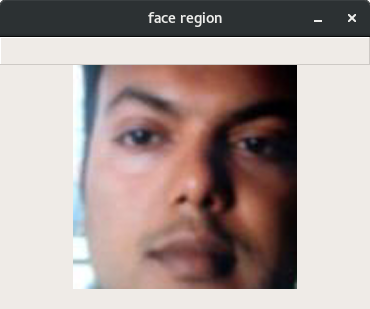
\includegraphics[width=.5\linewidth]{FaceExtraction.png}
                    \caption{This is the output produced from the preprocessing step of the ResNet based method.}
                    \label{FaceExtraction}
                \end{figure}
                
            \subsubsection{The Model}
                    
                \begin{figure}
                    \centering
                    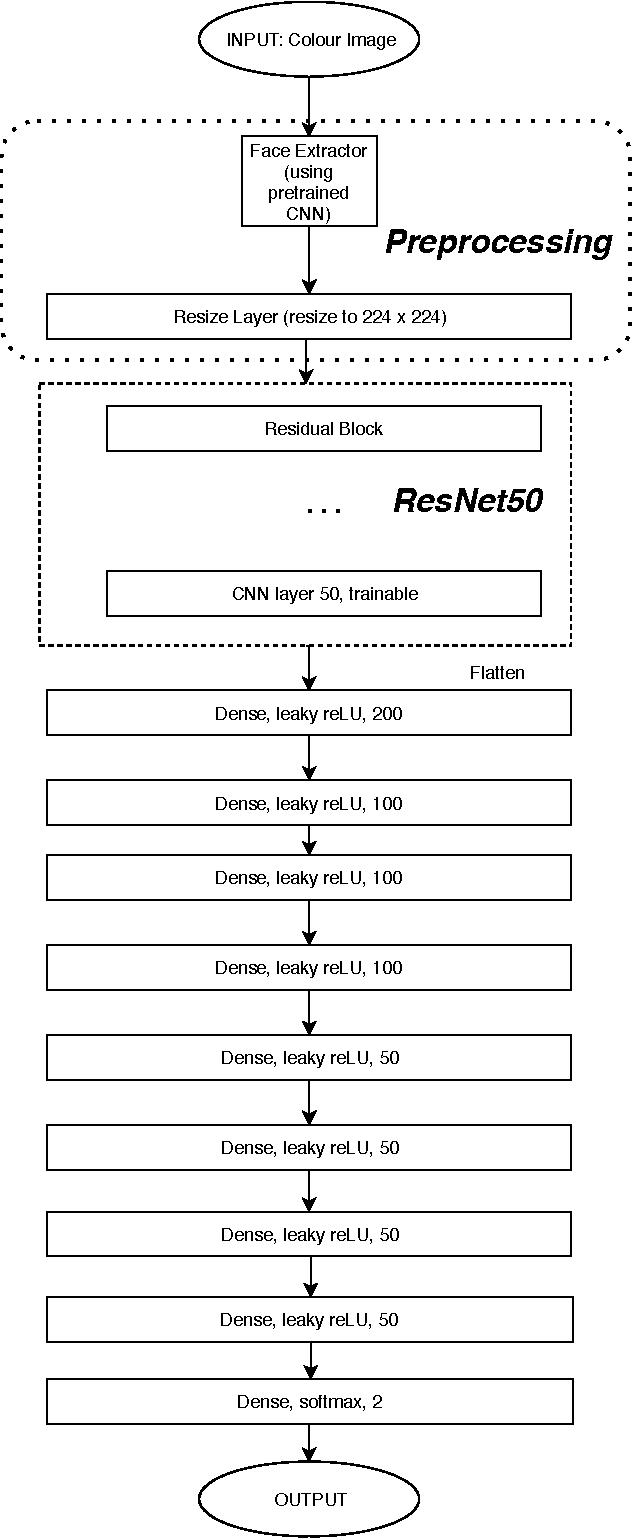
\includegraphics[width=0.3\linewidth]{2DCNNArchitecture.pdf}
                    \caption{The 2D CNN test architecture. We take the face image, resize to a fixed size, and put through ResNet50. The two last CNN layers
                    of this ResNet are trainable. The output of this network is flattened and fed through a deep feed forward network, yielding one output (which is the
                    liveness score as before).}
                    \label{2DCNNArchitecture}
                \end{figure}


                \paragraph{AlexNet}
                Initially, an AlexNet based classifier was designed. While AlexNet performance on the ImageNet dataset isn't as high as other models, it provided an ideal starting point to understand the difficulty
                of the classification. It was eventually found that AlexNet performed relatively poorly on facial liveness classification, and therefore a switch was made to a more complex and better performing model.

                \paragraph{Residual Networks}
                Residual Networks were chosen over VGG and Inception due to their better performance on ImageNet, coupled with their ability to be easily deployed without excessive memory/computation requirements.
                A ResNet 50 architecture was decided upon, as 50 layers seemed reasonable in terms of the available computational power that was available for this proof of concept. It was deemed that if ResNet 50 works, then ResNet 101 might perform equally, if not
                slightly better. A ResNet 50 architecture is an ideal proof of concept.

                While training a model from scratch might have advantages for some applications, a pretrained ResNet50 model from the Keras standard library was used. This was done due to the fairly small amount of data
                available (and therefore using a pretrained model can avoid overfitting), and also to save time learning the basic features that are present in all generic image classification models. Training the entire
                ResNet50 model would require a large number of parameters to be adjusted, so to further reduce the complexity of the training process, only the last layer was set to trainable, with the other layers remaining static.


                \paragraph{Feed Forward Classifier}
                While a CNN is ideal for processing images, a fully convolutional approach to classification didn't seem appropriate. The output from the ResNet 50 model was flattened, and fed directly into a feed forward neural network.
                While pooling layers were considered, these only take the maximum/minimum/average of specific sections, reducing the dimensionality, and the loss of data means the feed forward layer has less information to act upon. Therefore,
                it was instead decided to use no pooling layers. The output from the ResNet is flattened, and fed into an 8 layer feed forward neural network directly. The first layer of this network has a very large number of nodes,
                while the number of nodes is reduced towards the network output.
                
                With the initial experiment, the output layer consisted of a single node, with a sigmoid activation function. The entire network was trained using a binary cross-entropy loss function. The network accuracy yielded was fairly reasonable,
                but the confusion matrix showed that the model was outputting \emph{0.0} (fake) for each value, no matter the input. This was a problem, as the network wasn't suitably learning the dataset. As a result, three changes were made to solve the problem, which are outlined below.
                
                \paragraph{The Problem with Activation Functions}
                Initially, the \emph{reLU} activation function was used on all internal nodes within the feed forward network component. While reLU is very popular for improved speed over traditional activation functions such as tanh and sigmoid,
                for negative values it has a problem. ReLU is positive for all positive values, but 0 for all negative values.

                While all inputs were non-negative, weights could lead to these values becoming negative. There is a known problem called "dying ReLU", where some neurons output 0
                due to having a negative input (the weights and inputs for all input neurons sum to a non-positive value). Therefore, the model was able to learn 0 (fake) easily, but
                couldn't learn real (1.0) at all. \cite{liu_liu_2017}

                This problem was counteracted by changing activation function from reLU to Leaky ReLU. Unlike reLU, leaky reLU isn't zero when negative. It requires an input value $\alpha$, which is used
                as the gradient of the line when less than zero. \cite{liu_liu_2017} For this model, $\alpha=0.3$. The activation function is defined formally as:
                
                \begin{equation}
                    Activation(x) =
                    \begin{cases}
                    x, & \text{if}\ x>0 \\
                    \alpha \cdot x, & \text{otherwise}
                    \end{cases}
                \end{equation}

                \paragraph{The Problem with a Single Neuron Output}
                In order to mitigate the problem of outputting all zeros, the output method of the network was changed. Instead of a single neuron, giving a realness value, two neurons were used.
                These neurons would use the softmax activation function, rather than the sigmoid activation function, to ensure the sum of the neuron outputs would be zero (therefore giving a probability that can be used).
                The use of two neurons to encode the realness means that the nature for a network to learn 0 is slightly removed, as there will always be a non-zero output for one of the neurons expected. The encoding method used here
                is called one-hot encoding in the literature.

                \paragraph{Normalization and Dropout}
                Batch Normalization and dropout were both used within the feed forward network component to improve learning and reduce the risk of overfitting. Overfitting was a concern due to the small dataset that was used for training.
                Batch Normalization layers were added between each dense layer, which resulted in increased accuracy of the model.

                Throughout the experimentation process, the model was found to be overfitting. Therefore dropout was added (with a dropout level of 0.3) between each dense layer. This reduced the effects of overfitting.

                The overall outcome is shown in Figure \ref{2DCNNArchitecture}. The normalization and dropout are not visible in the diagram, since they are only used for training.


            \subsubsection{The Training Process}
                \paragraph{Optimizer}
                Initially, the Standard Gradient Descent was used as the optimizer. This was chosen due to the findings of \cite{SGDBetterThanAdamForImageClassification},
                which advised that SGD was better than the Adam optimizer for producing models that generalize. However, after experimenting further the Adam optimizer appeared
                to generalize better for this project. Using the SGD optimizer, the validation accuracy fluctuated with fairly poor accuracy results overall. The Adam optimizer
                didn't fluctuate, and the accuracy yielded was much higher.

                It's possible that SGD might perform better over longer periods of time with a very small learning rate, but due to time constraints and the need to experiment and show a proof of concept,
                Adam proved better for the purposes of this project.


                \paragraph{Loss Function}
                    Initially, while the model had a single neuron output, the binary cross entropy loss function was used as it's suitable for a single binary output.
                    However, when the two neuron output model was introduced, the loss function was changed to use categorical cross entropy as this was the most suitable
                    for a categorical one hot encoding method.

                \paragraph{Data Generators}
                    Due to the large amount of data being processed, it was necessary to use a data generator to conduct the preprocessing on the fly. While the preprocessing
                    could have been saved to disc, the preprocessing steps were changed throughout the project, therefore defeating the benefits of such an optimization.

                    Initially, Keras' built-in ImageDataGenerator was used, as it allowed for a preprocess function to be passed in. While this works for a preprocess function that yields the same shape image
                    as was input, Keras' ImageDataGenerator does not support resizing images within the preprocess function (e.g. for cropping).

                    Initially, a Lambda expression within the network was used to resize the image, but this led to problems with saving/loading models (due to Tensorflow being necessary).
                    Therefore, a custom data generator was written from scratch. With this new generator, it wasn't necessary to follow this size constraint within the preprocess function.


    \subsection{3D Face Reconstruction Liveness Test}
        \subsubsection{Overview}
            While 2D methods work well for traditional paper/screen based attacks, they are not designed for detecting the wearing of 3D masks. With 3D printing
            becoming more common, and automatic mask generators also becoming available online, this type of attack is becoming more common.

            The method proposed merged recent developments in facial reconstruction with recent deep learning models for classifying 3D data, to investigate a proposed
            architecture for a 3D classifier. Unlike previous methods, face data is captured in 2D using a standard device camera, before being reconstructed and then classified.

        \subsubsection{2D Image Preprocessing}
            The 2D preprocessing step followed a similar process to the previous liveness test proposed. A CNN based face detector produced a set of bounding boxes, and a square face image was produced
            following the same method as was proposed previously. Unlike the previous method, the image was resized to a fixed size of (192, 192) in color. This size was necessary due to the requirements
            of the pretrained model.

        \subsubsection{3D Facial Reconstruction}
            A method of obtaining facial structure from a 2D image was required. While video based methods such as Structure From Motion exist, they require a video input which has a large variety in motion, which might not be available/obtainable.
            However, recent research has developed a method known as VRN, which is a neural network designed to produce 3D facial structure from a single 2D image. \cite{3DReconstructionMethod}
            While the original work was built using the Torch deep learning framework, a pretrained model with appropriate source code exists for Keras. \cite{VRNTorchToKeras} This pretrained model
            takes an image of size (192, 192) in, and produces a 3D voxel based representation. 

            In order to correctly modularize the system, the \emph{FaceVoxelBuilder} class was produced to correctly load the pretrained model, and build the voxel structure for either 1 image, or multiple images (in the case of batch training).

            While implementing this component of the system, there was a problem: Tensorflow didn't build the objects from the pretrained model correctly in some cases, as certain components of the model didn't exist on the graph. This was solved by manually creating the predict function by calling a private helper function (\emph{model.\_make\_predict\_function()}).
            This was a known issue with the version of Keras that was being used, and the solution found was specified by the developers of the framework. \cite{KerasVoxNetBug}

        \subsubsection{3D Classification}
            While 2D image based classifiers exist, and perform well, this isn't the case with 3D image classifiers. A VoxNet based classifier was chosen due to the adequate performance on the SUOD dataset (of 69\%),
            coupled with the relatively small model size. \cite{VoxNetModel} While this model can in future be improved and adjusted, this classifier was believed to produce results that could show a proof of concept,
            and determine whether this method would be suitable for a web-based liveness system. The final architecture is shown in Figure \ref{3DClassifierArchitectureDiagram}.

            \begin{figure}
                \centering
                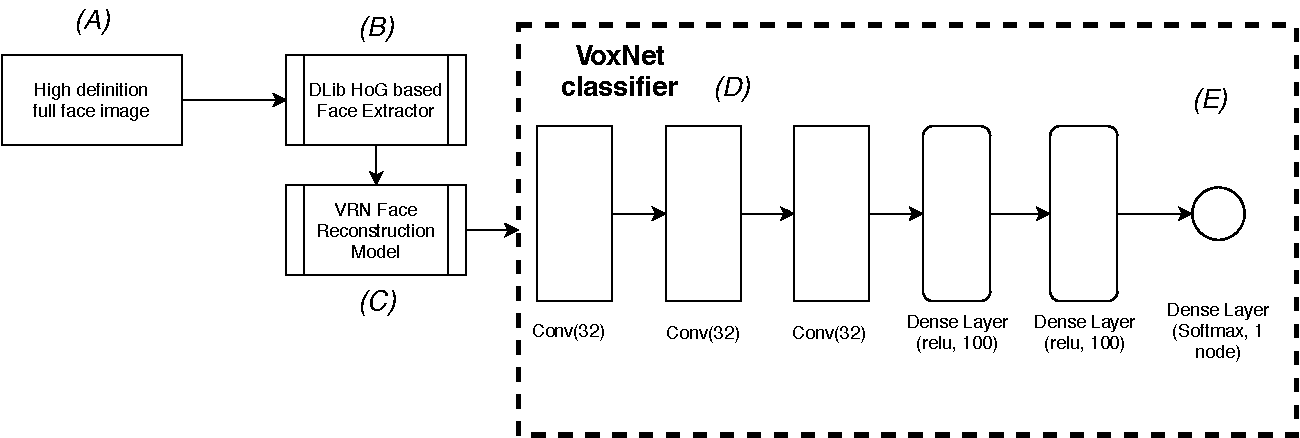
\includegraphics[width=\linewidth]{voxnet.pdf}
                \caption{
                    This is an overview of the 3D classifier. \textbf{(A)} a high resolution image is input into the classifier. \textbf{(B)} The image goes through a HoG based face detector. The bounding box of the face is extracted, and the image is cropped. 
                    The image is then resized to be 192x192 pixels, which is what's required by the VRN process.
                    \textbf{(C)} The pretrained VRN face reconstruction model takes an image input, and outputs a voxel representation. Some preprocessing from the VRN model 
                    is necessary to convert an occupancy grid into a voxel representation (this is done here rather than in the VoxNet model).
                    \textbf{(D)} The VoxNet classifier uses several 3D convolutional layers, along with a couple of Dense layers to classify.
                    \textbf{(E)} The output of the last dense layer is simply a single number defined as the certainty of realness. 1.0 implies the model is certain that the input is real, while 0.0 implies the model is certain that the input is faked.
                }
                \label{3DClassifierArchitectureDiagram}
            \end{figure}

        \subsubsection{The Training Process}
            Training was conducted using a binary cross-entropy loss function, with an Adam based optimizer. Binary cross entropy was used since there was only a single output node,
            compared with a categorical approach. 

            In order to conduct training, a Data Generator was used to minimize memory constraints, since the entire dataset didn't need to be loaded into memory after being preprocessed. Instead,
            only a single batch would be preprocessed on the fly, thus reducing memory usage considerably.

            While training, a problem with the built in data generators was encountered. While 2D images were being input, a 3D representation was required as output from the data generator,
            something that the Keras ImageDataGenerator wasn't able to deal with. Initially, the VRN model was included as part of the classification model. This would see a 2D image being input into the model,
            and the model would reconstruct to 3D and classify all in the same model. While this is a more monolithic approach, it would avoid the need to switch out the ImageDataGenerator. However,
            when implemented this didn't work: the 3D reconstruction process required non-tensor operations (more specifically, the use of the stack command), which could not be included as a network layer.

            Therefore, the final solution was to instead conduct the 3D reconstruction as a preprocessing step, and led to the replacement of the Keras ImageDataGenerator with a custom generator, designed to output 3D from 2D input.
            This custom generator would resize the images, reconstruct the 3D representation, and return the appropriate batch yielded. This solved the problem.

        \subsubsection{The Dataset}
            Unlike the previous two liveness tests, this liveness test relied on a completely different dataset, the Mask Attack Dataset (MAD). \cite{3DMadDataset}
            The goal of this liveness test was to detect mask based attacks (and more widely, 3D based attacks), and this dataset was used due to it being more representative of the problem
            than the Replay-Attack and NUAA datasets (which are designed for 2D based attacks).

            Unlike the 2D based methods, two datasets weren't used in a cross validation style assessment of the method, so instead the MAD dataset was split by subject (the person being spoofed):
            half of the subjects were used for the training/validation sets, and the other half were left for training purposes.

            Subjects 1,2,3,4,5,6,7 were used for training purposes, and 8,9,10,11,12, 13 were used for testing purposes. Splitting up the dataset in this way was necessary to correctly assess the classifier,
            to ensure results give a true indication of how well the model learned the features, rather than how well the model learned the dataset.

    \subsection{Consolidation Layer}
        Each liveness test individually might have some degree of error. Merging the results of each metric together into some classifier to produce a more reliable outcome would be ideal.
        While probability based methods (such as Bayesian calculations) would be feasible, this only works for a larger number of liveness tests. In some cases, very few liveness tests (minimum 2)
        might be used. 

        The solution proposed is to use a classifier, pretrained with the results yielded from the previous liveness tests. After training, this consolidation classifier would be able to spot patterns
        between each liveness test, and hopefully yield a better result by fusing the results of each individual test together. 

        \todo{Implementation DETAIL NEEDED!}


  
\section{Results}
    % based on the solution, what results did we yield? What did we find out?
    For both liveness tests, cross dataset validation/testing was conducted. Each model was trained using the entire NUAA dataset, and the Replay-Attack test set
    was used to measure the results shown below. In the case of the 2D Convolutional Neural Network (CNN), a validation set was required to ensure the model performed
    well, so in this case the Replay-Attack devel set was used. It must be noted that no overlap occurs between the Replay-Attack devel and test sets, to prevent the risk
    of these results being invalid. In order to visualize the result as a demonstration, a script was written using OpenCV calls to produce an overlay on top of the image.
    The results of these models in a faux-production environment can be seen in Figure \ref{SystemWorkingScreenshots}. 
    \begin{table}[ht]
        \centering
        \begin{tabular}[t]{lcc}
            \toprule
             & \textbf{Image Quality Liveness Test} & \textbf{2D CNN Liveness Test}\\
             \midrule
            \textbf{Accuracy (\%)} & 87.0 & 71.2\\
            \midrule
            \textbf{True Negatives (\%)} & 37.5 & 71.5\\
            \textbf{False Positives (\%)} & 12.5 & 1.37\\
            \textbf{False Negatives (\%)} & 0.5 & 22.5\\
            \textbf{True Positives (\%)} & 49.5 & 4.69\\
            \bottomrule
        \end{tabular}
        \caption{Table of results, showing test accuracy with the percentage of test results falling into the specific category defined in the confusion matrix (obtained using sklearn).}
        \label{ResultsTable}
    \end{table}

    \begin{table}[ht]
        \centering
        \begin{tabular}[t]{lcc}
            \toprule
             & \textbf{Image Quality Liveness Test} & \textbf{2D CNN Liveness Test}\\
             \midrule
            \textbf{Time to load (s)} & 0.00104 & 7.44\\
            \textbf{Time to classify 1 image (s)} & 1.40 & 1.04\\
            \bottomrule
        \end{tabular}
        \caption{Table of results, showing the wall clock time for the load and predict phases of both liveness tests.}
        \label{WallClockResultsTime}
    \end{table}

    \begin{figure}
        \centering
        \caption{Outputs from the \emph{live\_webcam\_output.py} file, being run on two different videos from the Replay-Attack test dataset. The model predicted the correct output here.}
        \label{SystemWorkingScreenshots}
        \begin{subfigure}[t]{.4\textwidth}
            \centering
            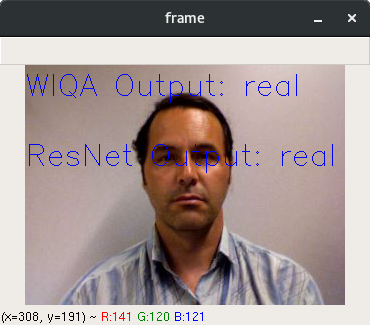
\includegraphics[width=\linewidth]{BothRealAndCorrect.png}
            \caption{The system correctly predicting a real piece of data. Image is from a video in the Replay-Attack test dataset.}
            \label{RealScreenshot}
        \end{subfigure}
        \hfill
        \begin{subfigure}[t]{.4\textwidth}
            \centering
            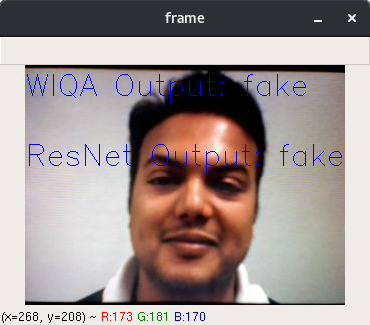
\includegraphics[width=\linewidth]{FakeOutputAndCorrect.png}
            \caption{The system correctly predicting spoofing in the input video. Image is from a video in the Replay-Attack test dataset.}
            \label{FakeScreenshot}
        \end{subfigure}
           
   \end{figure}
    \subsection{Testing Process}
        \subsubsection{Datasets}
            The Replay-Attack test dataset was used to access the results of each liveness test. This dataset contains no overlap with the set that was trained on, therefore ensuring that
            the results are a true indication of the generalised performance.

        \subsubsection{Accuracy}
            Top-1 accuracy is an ideal metric to judge the performance of the system, since a high Top-1 accuracy in the results would show how often the liveness test yields the correct results.
            
            A Top-1 accuracy figure of 50\% implies that the model is simply randomly yielding output (since there are two cases), which isn't ideal. A figure of 70\% implies that the model
            is reasonably yielding the correct result and is feasible, but might need minor changes or more training to yield a better result. A figure of over 85\% implies that the model
            is yielding the correct results most of the time. The higher the accuracy figure, the better, when being run on an unseen dataset.

        \subsubsection{Confusion Matrix}
            While accuracy is a reasonable metric, it's also important to visualise how often each model selects each case (fake/real), and whether the selection is correct or incorrect.
            There are four important terms with the confusion matrix. These are:

            \paragraph{True Positives}
                This is the percentage where the model predicts that an input is real, where the input is real. Therefore, the liveness test has identified a user as real correctly.
                This figure should be above zero, and a reasonable figure. 

            \paragraph{False Positives}
                This is the percentage where a model predicts an input is real, where the input actually contains a spoofing attack. This is a concern, since for a security focused
                liveness test, this should be mitigated as much as possible.

            \paragraph{True Negatives}
                This is the percentage where a model predicts an input is fake, where the input contains a spoofed image. This is an indication of how often a model predicts that an input is faked.
                This again should be reasonably high.

            \paragraph{False Negatives}
                This is the percentage where a model predicts an input is fake where it's actually real. This isn't ideal, but this is the preferred option when a liveness test performs poorly, since
                this would only cause inconvenience for the user, rather than a potential security breach.
            
   
    % CNN table: 4317 & 83 & 1357 & 283
    \subsection{Image Quality Liveness Test}
        Overall, the Image Quality Test performed as expected with reference to the initial paper. Unlike the original paper however, instead of isolating the face
        from the input image, the entire image was used. While isolating the face might perform well, using the entire image might provide further subtle information
        about the image quality.

        The overall results, shown in Table \ref{ResultsTable} show fairly good performance on the Replay-Attack test dataset, with an accuracy of 87\%. This is in line with
        what was expected from the paper \cite{ImageQualityAssessmentTest}. While accuracy gives an overall account of the results, it doesn't show the overall performance.
        
        The level of true negatives and true positives respectively are fairly high, but the number of false positives was slightly higher than expected (i.e. where the model predicts someone to be real where they are actually not).
        What's interesting to note is the low number of false negatives (indicating someone is fake where they are real), which in our security conscious case isn't wanted (since inconvenience isn't as much of a problem as security).
        However, the overall performance was better than expected.
        % Total results - the RAW data in case people need it.
        % 0.87
        % True Negatives:  75
        % False Positives:  25
        % False Negatives:  1
        % True Positives:  99
        While accuracy is important, the time taken for the model to classify a single image is also important. The LDA method took 1.40 seconds to classify a single 2D image, which is within the specified 2 seconds bound.
        Also, the model itself is very small and therefore can be loaded in a very minute amount of time (0.001 seconds). The bulk of the time required is in the calculation of the metrics, rather than the classification process,
        and therefore future speed optimizations could consider improving the calculation of the metrics. These results can be seen in Table \ref{WallClockResultsTime}.

    \subsection{2D Convolutional Neural Network Liveness Test}

        The overall performance of our liveness test can be seen in Table \ref{ResultsTable}. While not as accurate as the previous model, the model still detects true negatives with a fairly high percentage.
        While the overall accuracy of this model could be improved with further training or by deepening, the results show that this basic architecture is feasible. In the security conscious environment of facial liveness,
        false negatives, while potentially annoying to the end user, are an ideal result compared to false positives (which would imply that someone is real when they are fake). While false positives still exist, their number is small compared to the number of negatives.
        Furthermore, the number of positives is small, meaning that this model leans on the side of caution, something that is ideal. Therefore, this model would be secure and accurate enough with further training (and potentially replacing ResNet50 with a deeper ResNet model).

        The time taken to load the model from memory was the main bottleneck in terms of computational performance, as loading the model into memory for the first time took 7.44 seconds. However, once the model was loaded,
        the time taken to predict a single image is very small, on average taking 1.04 seconds, which is even smaller than the W-IQA test, and almost half the specified 2 second time, which is ideal. These results can be seen in Table \ref{WallClockResultsTime}.     
        % Confusion Matrix = [[4317  283]
%           [1357   83]]

    \subsection{3D VoxNet Liveness Test}
        This method had some major performance challenges. The 3D facial reconstruction worked well, producing the desired outcome. However, the 3D classifier (VoxNet), had numerous problems.
        The original VoxNet model, proposed in \cite{VoxNetModel}, used 32 filters for the Conv3D layers (with a 32x32x32 input). However, using 32 filters in our model for each Convolutional Layer (alongside the larger data input than expected),
        led to memory errors and wasn't able to be trained on the training hardware.  Reducing the 3D reconstruction resolution wasn't an option, since the entire model would require retraining (which would take lots of time, resources, and wasn't feasible).
        Furthermore, as seen with the 2D CNN method, reducing the resolution might also reduce the accuracy. Therefore, the remaining solution was to reduce the number of filters down to a small 12 filters per convolution layer.

        During the training process, with a variety of learning rates, the accuracy of the model didn't leave 50\% with a differing amount of batch sizes. This indicates that the model wasn't learning the features correctly (potentially due to the lack of filters in the Convolutional Layer).
        
        While the classifier itself didn't work and yield any meaningful results, it's also important to consider the time taken for a 2D image to be reconstructed. 
        To reconstruct a single image from 2D to a 3D face structure, it took 5.39 seconds, which already exceeds the 2 second constraint set by the specification.

        Due to the poor accuracy with a low number of filters, the excessive amount of memory required for unknown accuracy results, and the large time taken to reconstruct the 3D structure (not including the added time to theoretically classify the result),
        this liveness test clearly isn't feasible for the purpose of a web liveness service.

    \subsection{Consolidation Layer}
        
        \begin{figure}
            \centering
            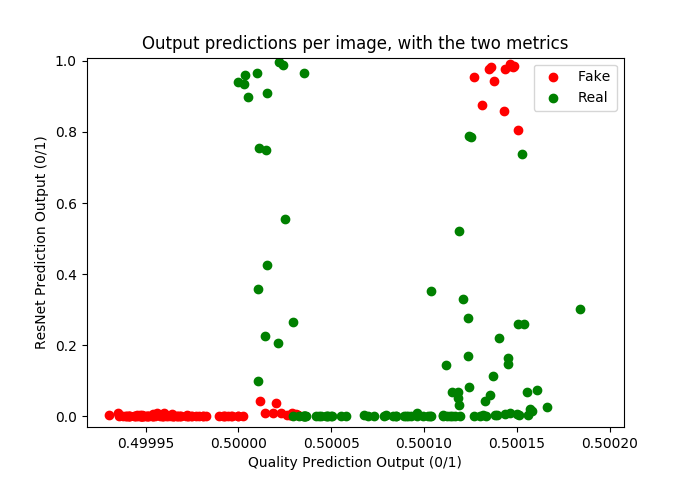
\includegraphics[width=.5\linewidth]{LinearlySeparable.png}
            \caption{A plot of ResNet output against WIQA output. As one can see, for two metrics a perceptron could be used due to the linearly separable nature of the data (that is, a single line could be used to
            separate the real and fake classifications in some cases). Effectively, with two metrics this would be acting as an OR gate (with fuzzy calculations).}
            \label{LinearlySeparableGraph}
        \end{figure}
    
        As shown in Figure \ref{LinearlySeparableGraph}, plotting the results together with the probability outcome (rather than the class outcome),
        yield a plot where the two classes could approximately be divided up with a single line. Therefore, as expected, the relationship between predictions is
        linearly separable.

        While investigating this further, using an LDA as a consolidation layer yielded fairly ideal results: 75\% accuracy to be precise. 
        \todo{LDA: confusion matrix}

        However, it's important to note that while this works for two liveness tests, we can't test this method for a larger number of liveness tests. While accuracy was fairly reasonable,
        using more metrics could yield improved accuracy.

    \subsection{Live Application}
        While numerical figures are useful to measure the results, it's also important to show performance on a completely unseen subject (through the use of a webcam). An OpenCV based script was
        written to, in real time, access the output of the liveness tests and overlay the results on the screen with their predictions. 

        The successful results can be seen in Figure \ref{SystemWorkingScreenshots}. While not numerical, it yielded a large number of useful insights into the real time nature of such a system,
        and it's practical deployment.

        \paragraph{Benefits of CNN facial isolation}
        The CNN facial isolation was found to be very good at selecting the facial area ready for preprocessing. Even with part of the face covered up, it still yielded a reasonable
        facial crop, which could then be fed into the network. Also, the head being placed at different angles also yielded a reasonable face isolated image that could be used for the
        CNN metric.
    
        \paragraph{Resolution problems with WIQA test}
            While the test datasets contain a small number of different resolutions, the differences in resolutions are minimal. Therefore, using a completely different image resolution
            of 1280x720, which was completely unseen by the classifier previously. This led to the model predicting each input as real, which was incorrect.

            The solution taken was to resize this image down to a more reasonable 640x480, which yielded far better performance in real time. However, in future iterations, resolution is
            a factor that needs to be considered, and potentially the resolution should be included in the classified vector. Furthermore, more resolutions should be tested to yield a reasonable
            classification.

        \paragraph{Uncertainty of the CNN liveness test}
            While the CNN liveness test could correctly classify a specific facial input, it would occasionally change the prediction to an incorrect prediction
            as frames were stepped through. This was even observed with minimal change in the input image. Since the prediction of 1 image takes minimal time,
            it might be ideal in future to take a set of 8 frames, and output the mode classification from this batch, this way smoothing out the prediction.
            Alternatively, the CNN liveness test might need more training to assert the difference between real/fake in a more varied set of lighting conditions and resolutions.
            \todo{Show uncertainty here somehow}

        \paragraph{Problem in running liveness tests in series}
            Since we have two liveness tests, the script runs the WIQA test first, before running the CNN based liveness test. This is fairly slow, as each liveness test requires their
            own resources and time to complete. It might be more ideal to parallelise this in future, to yield better performance. While single-computer parallelisation might not be the best option
            (since each classifier requires some degree of multithreading), multiple systems could be used to speed up this process.

\section{Evaluation}
    % How well our system works, how well did it assess stuff, and how it can be improved.
    % what are the uses of our research? e.g. influence and improve the design of xyz...
    \subsection{Usefulness of our system}
    
        % Identified two metrics that could be deployed.
        % Created the structure of such a system (e.g. consolidation layer) to allow for future extensions with further liveness tests.
        % Applications: within IoT devices, use within web browsers alongside existing face recognition services. 
        % There is an argument that one could steal your likeness and use it elsewhere on the internet. However, providing liveness tests
        % are suitable, there is no other way of stealing ones face. There would be a need to ensure furhter development of such a system.
        % Developing a single component as a service would mean developers could focus on developing their applications. 
        \paragraph{Quality Test}
            The Quality Test performed well, and is suitable for a web based liveness service due to the high 87\% accuracy achieved.
            True positives and true negatives (that is, correct predictions for both real and fake) were high which means that the classifier
            is classifying correctly. However, the high false positive rate shows a slight cause for concern, since the model in 12.5\% of cases
            classified a fake image as real, which isn't ideal for our security focused solution. This could potentially be solved by adjusting output
            variable of the classifier (using a figure representing 'fakeness' rather than realness). This would hopefully lead to more false negatives,
            which are inconvenient but more secure for the system.

            In terms of computational performance, a 1.40 second time for classifying a single image is within the limits of the expected 2 seconds, and could be improved further
            with parallel based methods, and not relying on libsvm for the BIQI metric.
        \paragraph{2D CNN}
            The 2D CNN Test performed adequately. While the accuracy was lower than expected (at 71\%), the classifier itself still performed better than random.
            Furthermore, the model was very good at classifying true negatives, with a total percentage of 71.5\% being true negatives. While the model itself had
            a higher than expected false negative percentage, this is just inconvenient for the user rather than a security problem. The model showed it could classify true
            positives, but this figure was fairly low. This could be improved by improving the training process: ensuring each input image has a correctly identified face (as
            some images without a detectable face would have been left to classify the entire image, just resized to the input size). The less noise in the input data, the better the potential
            results in the future. Furthermore, using a larger ResNet model, such as ResNet-101 could lead to better results.

            In terms of performance, classifying an image is very quick, but the time taken to load the model is what took the most time (due to memory needing to be allocated and written to).
            In production, providing a model was preloaded and ready to accept input, the computation time of this metric would be very fast, and therefore be ideal for inclusion in a liveness web service.
        
        \paragraph{3D VoxNet Liveness Test}
            As seen from the results, this method of liveness test isn't feasible. With extra training, while the accuracy of the model could be improved, the
            real time memory requirements don't seem feasible. Based on the VoxNet paper, the accuracy achieved with a 32x32 VoxNet classifier on the SUOD dataset (a 3D dataset of objects)
            is 69\%. While this accuracy could be justified with reasonable computational and memory characteristics, this further proves that this method isn't feasible in the current state. In the future, a new approach of detecting 3D attacks is necessary.
    
    \subsection{Improvements}
        \paragraph{Representing 3D Attacks}
        While our system works fairly well for 2D based attacks, performance for 3D based attacks definitely needs work.
        While our VoxNet based method didn't yield any meaningful results, there is a chance that a 2D image could yield results
        with 3D based attacks (using a residual network on a static image to detect minor mask-based imperfections), or alternatively
        considering a sequence of images using LSTMs to detect changes in movement. This however would require video input, meaning the
        NUAA dataset wouldn't be useful.

        \paragraph{Preventing Source-Quality Web Browser Attacks}
        Current approaches followed (including ones in this paper) assume that the video capture and liveness processing is conducted securely, 
        without any interference from malicious actors. However, in the case of web browsers, the video capture process might not be secure as
        the client-side code can be easily tampered with, and therefore shouldn't be trusted fully. The solution to this is a random video input,
        something requested by the server and required to be contained within the video (similar to a CSRF token in web forms). The answer to this
        is contained within an existing liveness metric: a motion based one. The process of face flashing would be ideal, as a specific color could
        be requested, and expected to be visible in the frame. Alternatively, head tracking and expecting a specific set of motions would also be suitable,
        but as this would require user input might not be favorable.

        % TODO might be a way of explaining tampering with getusermedia.
        
        \paragraph{Existing BIQI implementation}
        Currently, the BIQI implementation requires the use of a subprocess to call libsvm based commands on the system. Instead of using standard output, files are used which
        cause a reduction in speed.
        Speed isn't the only problem here, as scaling would become a problem due to the existing implementation. 

        To fix this problem, a reader would be needed to import a trained libsvm model into sklearn, and the code would then need to be refactored to use the updated sklearn model. 

        % \paragraph{Privacy/Legal Considerations}
        %     While the security of a facial liveness cloud service is reasonable, there would be some legal concerns to consider in the deployment of an actual application.
        %     Face data, as with all biometric data, is classed as sensitive personal data. This can be found in the GDPR definitions, from \cite{GDPRDefinitions}. As such, care would need to be taken in the development of such a system
        %     to ensure compliance. While the details below are not legal advice, these would be the starting point to building a liveness service that's more compliant.

        %     % Source: https://thenextweb.com/contributors/2018/10/29/heres-how-face-recognition-tech-can-be-gdpr-compliant/
        %     When designing such a service, collecting user consent is necessary through a positive opt-in (without any prefilled tick boxes). In addition to collecting consent, users must be able to withdraw their consent too.
        %     Naming any third parties might be necessary too, especially if using a Cloud-based service. Furthermore, some anonymisation process would need to be implemented to ensure that the image isn't easily identifiable (therefore names
        %     must not be recorded). Therefore, no user accounts of persistent storage tieing people to their faces would be ideal, to ensure anonymisation. While a facial liveness web system would be securing a facial recongition system, the 
        %     liveness system itself would need to be secure in order to meet GDPR regulations. \cite{GDPRForFacialRecognition} Encrypting data in transit is fairly easy, using SSL is a modern standard
        %     and certain browsers require the use of SSL for accessing certain media APIs. Encryption of data at rest might be necessary, but since the image wouldn't necessarily be stored that might not be required. 
            

        %     Aside from GDPR, licensing of datasets is another concern. The Replay-Attack dataset is licensed on condition of research, rather than for commercial use. 
        %     As such, the deployed version of such a liveness based system would need to use a network trained with a new dataset that has the appropriate licensing (either a bespoke one, or one that is public domain).

\section{Conclusions}
    % overall, what did the project show?
    % TODO this needs to probably be reworded.
    This project showed that creating a facial liveness service for the web is a feasible idea, and performs fairly well for 2D attacks, with adequate accuracy and computational requirements.
    The image quality liveness test is accurate and fast, while the ResNet based method is a feasible idea and performs adequately, and could be improved further to improve the accuracy. For 3D attacks however, the
    proposed VoxNet based model performed badly and is not recommended for inclusion in a liveness test web service.

    % In addition, the improvements to the existing system were shown, and potential GDPR considerations were shown on how to implement such a system to better comply with the regulation. In building of a system for commercial use, it's important
    % to note that licensing on training and testing datasets would require new datasets be used.

\printglossary
\bibliographystyle{abbrv}
\bibliography{report}

\end{document}